\documentclass[10pt]{beamer}

%%%
% PREAMBLE FOR THIS DOC 
%%%
%https://tex.stackexchange.com/questions/68821/is-it-possible-to-create-a-latex-preamble-header
\usepackage{/Users/miw267/Repos/csci246_spring2025/slides/preambles/beamer_preamble_for_CSCI246}



%%% TRY TO RESHOW TOC AT EACH SECTION START (with current section highlighted)
% Reference: https://tex.stackexchange.com/questions/280436/how-to-highlight-a-specific-section-in-beamer-toc
\newcommand\tocforsect[2]{%
  \begingroup
  \edef\safesection{\thesection}
  \setcounter{section}{#1}
  \tableofcontents[#2,currentsection]
  \setcounter{section}{\safesection}
  \endgroup
}


%%%% HERES HOW TO DO IT CORRECTLY
% FIRST IN .STY FILE, DO
%\usetheme[sectionpage=none]{metropolis}
% THEN AT EACH SECTION DO
%\begin{frame}{Outline}
%  \tableofcontents[currentsection]	
%\end{frame}



%\setbeamertemplate{navigation symbols}{}
%\setbeamertemplate{footline}[frame number]{}


%%%
% DOCUMENT
%%%

\begin{document}

%\maketitle

%% Title page frame
%\begin{frame}
%    \titlepage 
%\end{frame}





\title{Monday 01/27/2025: Boolean Algebra}
\author{CSCI 246: Discrete Structures}
\date{Textbook reference: Sec. 7, Scheinerman}

\begin{frame}
    \titlepage 
\end{frame}


\begin{frame}

\begin{myredbox}[title=New way to get quizzes back!]
Each student may line up either before class (2:00-2:10) or after class (3:00-3:10) to collect graded quizzes from the previous class from Fatima. \\
\vfill 
This will hopefully free up Fatima's time during class to assist with group exercises.
\end{myredbox}
\vfill \vfill 

\begin{myyellowbox}[title=Today's Agenda]
\begin{itemize}
	\item Reading quiz  (5 mins)
	\item Mini-lecture ($\approx$ 15 mins)
	%
	\begin{itemize}
	\item Review Friday quizzes. 
	\item Go over Sec. 6 group problems
	\end{itemize}
	%
	\item Group exercises ($\approx$ 25 mins)	
\end{itemize}

\end{myyellowbox}


\end{frame}



\begin{frame}{Reading Quiz}
 \begin{mygreenbox}[title=Reading Quiz (Sec. 7 - Boolean Algebra)]
Use a truth table to prove that the expressions $x \implies y$ and $(\lnot x) \, \lor \, y$ are logically equivalent.
\vfill 
\end{mygreenbox}
\vfill \vfill 

\begin{myredbox}[title=Notation reminder]
\begin{itemize}
\item $\implies$ means \texttt{implies}
\item $\lnot$ means \texttt{not}
\item $\lor$ means \texttt{or} 	
\end{itemize}
\end{myredbox}
\end{frame}


\section{Mini-lecture}



\begin{frame}{Feedback on your reading for Sec. 6 (counterexample)}

\begin{myyellowbox}[title=Poll]
Is the following statement true or false? 
\[ -5|5 = -1 \] 
\end{myyellowbox}

\pause 

\begin{myredbox}[title=Alert!]
In mathematical reasoning, you always need to \textbf{refer back to the definitions}.    
\end{myredbox}

\pause 
	\begin{mydef}[title=Reminder of Definition 3.2 (\textbf{Divisible})]
	Let $a$ and $b$ be integers.  We say that $a$ is \textit{divisible} by $b$ provided there is an integer $c$ such that $bc=a$. The notation for this is $b|a$. 
	\end{mydef}
\pause 
\footnotesize 
Solution to poll: The statement is \textbf{incorrect}! Why? \pause $-5|5$ is a \textbf{proposition}, so it can't equal $-1$. We would instead write just $-5|5$, or perhaps $-5|5 = \texttt{TRUE}$. How do we justify the proposition? \pause We have $-5|5$ because if $a=5$ and $b=-5$, there exists an integer (namely $c=-1$) such that $bc=a$.
\end{frame}

\begin{frame}{Feedback on Sec. 6 reading}

 \begin{mygreenbox}[title=Reading Quiz (Sec. 6 - Counterexamples)]
Disprove the following conjecture:  
\textit{Let $a$ and $b$ be integers.  If $a|b$ and $b|a$, then $a=b$.}   You can disprove the conjecture by providing a counterexample.  \textbf{Make sure to show that your counterexample satisfies the hypothesis (the "if" statement).} 
\vfill 
\end{mygreenbox}

\textbf{Common errors}
\begin{enumerate}
\item \textbf{Not justifying the counterexample.} Many people correctly gave a counterexample, e.g. $a=5, b=-5$, but did not justify why $-5|5$. 
\item \textbf{Incorrect use of notation.} Many people wrote $-5|5=-1$.  (However, I didn't take off points for this error.) 
\end{enumerate}
\end{frame}


\begin{frame}{Reading Quiz Scores}

\begin{figure}[ht]
        \centering
        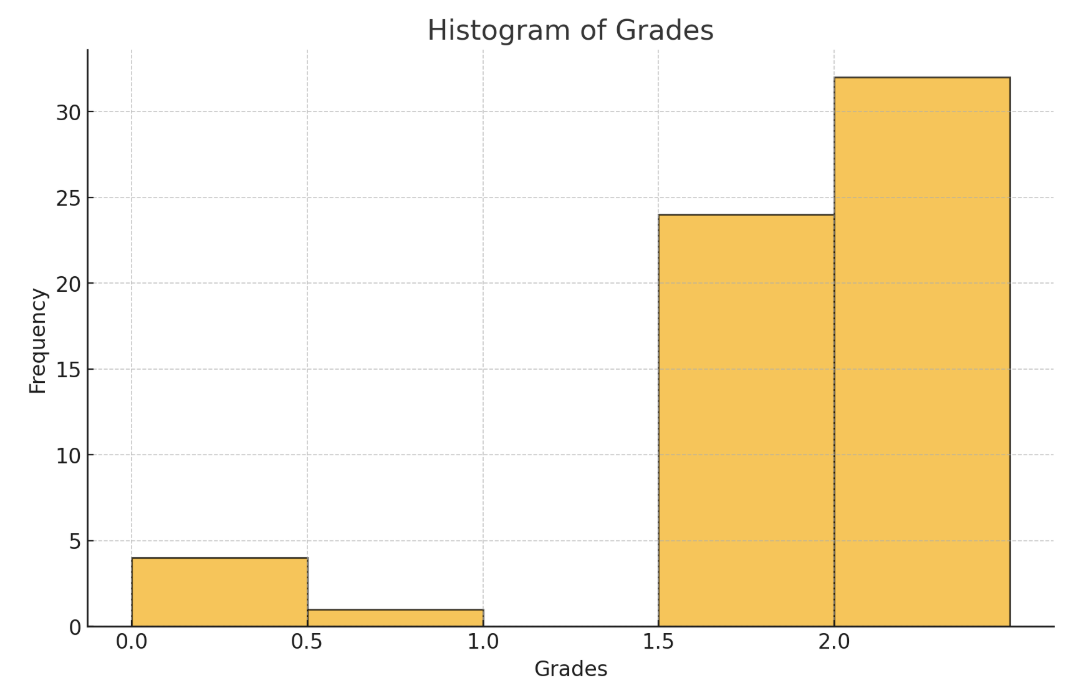
\includegraphics[width=\textwidth]{images/sec6_reading_scores}
        \caption{Reading Quiz (Sec. 6)}
        \label{fig:figure1}
\end{figure}
\end{frame}

\begin{frame}
\begin{figure}

\includegraphics[width=0.7\textwidth]{images/tips_for_reading_math}
\end{figure}
%
\begin{figure}
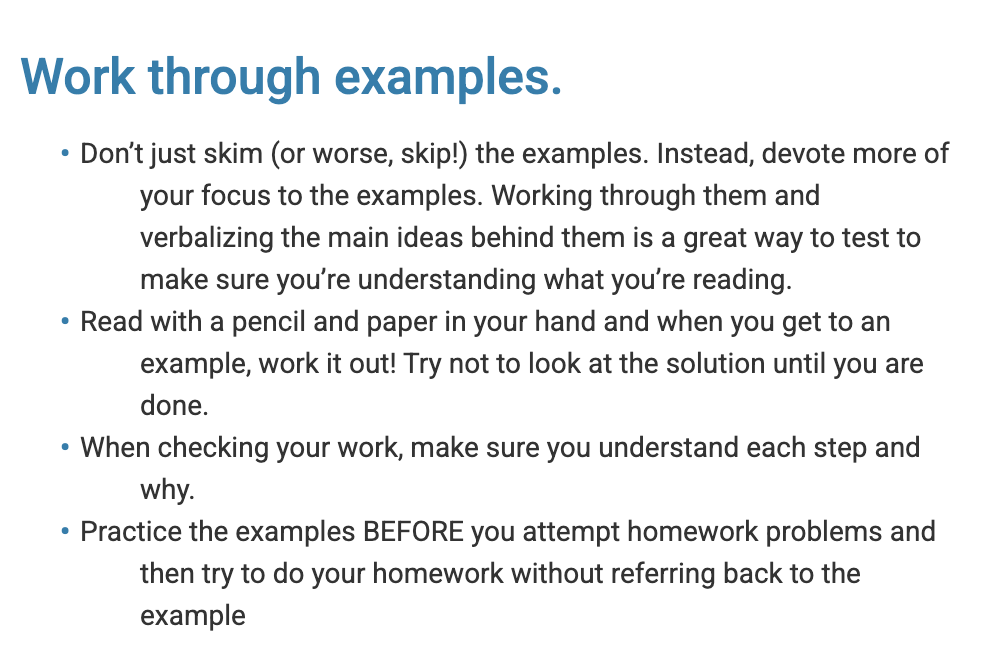
\includegraphics[width=0.7\textwidth]{images/work_through_examples}
\end{figure}
\bottomtext{\hfill Source: \url{https://learningcenter.unc.edu/tips-and-tools/readingmathtexts/}.}
\end{frame}


\begin{frame}{My solution to reading Quiz (Sec 6 - Counterexamples)}
\footnotesize 

 \begin{mygreenbox}
\footnotesize 
Disprove the following conjecture: \textit{Let $a$ and $b$ be integers.  If $a|b$ and $b|a$, then $a=b$.}
\vfill 
\end{mygreenbox}

\vfill \vfill 
\footnotesize 
%\textbf{Solution.} 

\begin{tabularx}{\textwidth}{|L{3cm}|X|}
\hline \textbf{Annotation} & \textbf{Main Text} \\ \hline
\hlorange{Structure} & \hlorange{Let $a=5$, $b=-5$. \\  First, we show that the hypothesis holds [i.e., that $(5|-5)$ and $(-5|5)$].}  \\
\hlgreen{Unravel defn.} & \hlgreen{$a|b$ means there is an integer $x$ such that $ax=b$.} \\
& \hlgreen{Likewise $b|a$ means there is an integer $y$ such that $by=a$.} \\
\hlred{The ``Glue"} & \hlred{Substituting for $a$ and $b$, we need to show that there are integers  $x$ and $y$ such that $5x=-5$ and $-5y=5$.   We see these equations hold by taking $x=-1$ and $y=-1$.} \\
\hlorange{Structure}  & \hlorange{Hence $5|-5$ and $-5|5$, so the hypothesis is met.} \\
\hline
\hlorange{Structure}  & \hlorange{Now we show that the conclusion fails [i.e. that $-5\neq5$.]} \\
\hlred{The ``Glue"} &  \hlred{This is immediately clear.} \\
\hline
\end{tabularx}
\vfill 
\textbf{Remark.} I scored out of 2 points, and gave 1.5 points for a correct counterexample, and 0.5 points for any argument that the hypothesis holds.
\end{frame}






\begin{frame}{An interesting question}

 \begin{mygreenbox}[title=Reading Quiz (Sec. 6 - Counterexamples)]
Disprove the following conjecture:  
\textit{Let $a$ and $b$ be integers.  If $a|b$ and $b|a$, then $a=b$.}  
\end{mygreenbox}
\vfill 
\begin{myyellowbox}[title=Poll]
Is $a=1, b=0$ a valid counterexample?
\end{myyellowbox}
\vfill 
\pause 
	\begin{mydef}[title=Reminder of Definition 3.2 (\textbf{Divisible})]
	Let $a$ and $b$ be integers.  We say that $a$ is \textit{divisible} by $b$ provided there is an integer $c$ such that $bc=a$. The notation for this is $b|a$. 
	\end{mydef}
\vfill 	
\pause 
\footnotesize 
\textbf{Solution to poll:} We have $a|b = 1|0$, since there is an integer $c$ such that $ac=b$ (that is, $1 \cdot c =0$). However, we do not have $b|a=0|1$, since there is no integer $d$ such that $bd=a$ (that is, there is no integer $d$ such that  $0 \cdot d = 1$). That is, the hypothesis doesn't hold, so the statement doesn't apply.  
\end{frame}






\begin{frame}{Problems Quiz Scores}

\begin{figure}[ht]
    \centering
        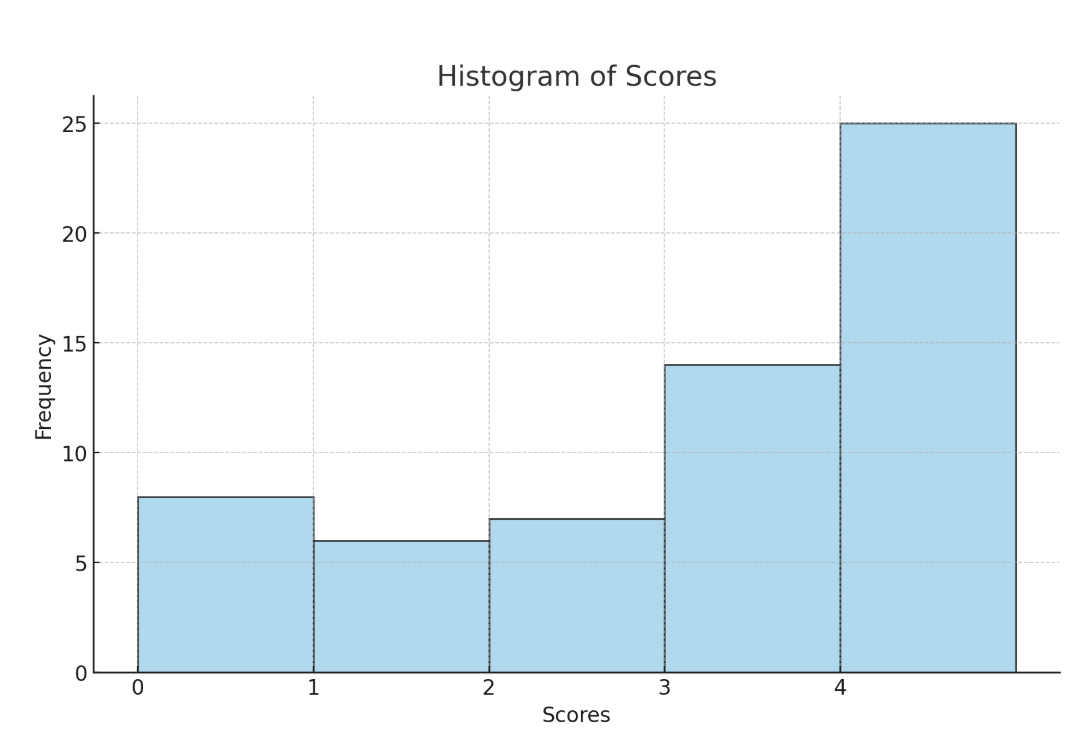
\includegraphics[width=0.7\textwidth]{images/problems_quiz_2025_01_24}
\end{figure}
\vfill 
\textbf{Most common error:} Most students with 3/4  correctly wrote the truth table columns for $A \implies B, B \implies A$ and $A \iff B$, but   but didn't argue why/how $A \iff B$ is identical to $(A \implies B) \, \alert{\texttt{and}} \, (B \implies A)$.  
\vfill 
\textbf{Solution:} The question was exactly a group exercise from Sec. 4 (Theorems).   See slides from that section for solution.
\end{frame}



\begin{frame}[standout]

\vfill 
\alert{Review solutions to Sec. 6 group exercises}
\vfill

\end{frame}









\begin{frame}[standout]

\alert{Sec. 7 (Boolean algebra) group work!}
\vfill
Students are randomly assigned into groups of 3 on the next slide.
\vfill 
Each group gets $\half$ of a white board.
\vfill
If the  $\half$ white board is inconvenient, feel free to write on a window! 
\end{frame}

\begin{frame}
\footnotesize
Group 1: justice.mosso,owen.obrien,nicholas.harrington1\\
Group 2: joseph.triem,connor.yetter,anthony.mann\\
Group 3: peter.buckley1,evan.barth,jeremiah.mackey\\
Group 4: devon.maurer,carsten.brooks,jacob.ketola\\
Group 5: kaden.price,michael.oswald,blake.leone\\
Group 6: emmeri.grooms,griffin.short,carver.wambold\\
Group 7: caitlin.hermanson,connor.mizner,connor.graville\\
Group 8: jack.fry,samuel.mosier,tyler.broesel\\
Group 9: ethan.johnson18,lucas.jones6,conner.reed1\\
Group 10: micaylyn.parker,peyton.trigg,jacob.shepherd1\\
Group 11: samuel.hemmen,cameron.wittrock,nolan.scott1\\
Group 12: yebin.wallace,alexander.knutson,colter.huber\\
Group 13: pendleton.johnston,reid.pickert,jada.zorn\\
Group 14: luke.donaldson1,joseph.mergenthaler,jonas.zeiler\\
Group 15: ryan.barrett2,william.elder1,samuel.rollins\\
Group 16: jacob.ruiz1,aaron.loomis,lynsey.read\\
Group 17: zeke.baumann,delaney.rubb,james.brubaker\\
Group 18: erik.moore3,derek.price4,sarah.periolat\\
Group 19: alexander.goetz,tristan.nogacki,jett.girard\\
Group 20: mason.barnocky,jakob.kominsky,luka.derry\\
Group 21: julia.larsen,bridger.voss,evan.schoening\\
Group 22: john.fotheringham,adam.wyszynski,matthew.nagel, timothy.true\\
\end{frame}


\begin{frame}{Group exercises}
\footnotesize 
\begin{enumerate}
	\item DeMorgan's laws are:
	\[ \lnot (x \land y) = (\lnot x) \lor (\lnot y) \quad \text{and} \quad \lnot (x \lor y) = (\lnot x) \land (\lnot y) \]
	Prove the first of these (using truth tables). Then use DeMorgan's law to show how to disprove an if-and-only-if statement.
	\item A \textbf{tautology} is a Boolean expression that evaluates to \texttt{TRUE} for all possible values of its variables.  For example, the expression $x \lor \lnot x$ evaluates to \texttt{TRUE}  both when $x=\texttt{TRUE}$ and $x=\texttt{FALSE}$.  Use truth tables to show the following are tautologies:
	    \vspace{-0.5cm}
		\begin{enumerate}
		\item[(a)] $(x \lor y) \lor (x \lor \lnot y)$
		\item[(b)] $x \implies x$
		\item[(c)] $\texttt{FALSE} \implies x$
		\item[(d)] $(x \implies y) \land (y \implies z) \implies (x \implies z)$ 
		\end{enumerate}
	\item  A \textbf{contradiction} is a Boolean expression that evaluates to \texttt{FALSE} for all possible values of its variables.  For example, the expression $x \land \lnot x$ is a contradiction.  Use truth tables to show that the following are contradictions:
		\begin{enumerate}
		\item[(a)] $(x \lor y) \land (x \lor \lnot y) \land \lnot x$
		\item[(b)] $x \land (x \implies y) \land (\lnot y)$.
		\end{enumerate}
	\item Reprove the items in \#2 and \#3 using the properties in Theorem 7.2 and the fact  from Prop 7.3 that $x \implies y$ is equivalent to $(\lnot x) \lor y$.
\end{enumerate}
\end{frame}


\end{document}
